
\documentclass[landscape, DIV=99, 14pt]{scrartcl}

\renewcommand*{\familydefault}{\sfdefault}

\RequirePackage{graphicx}
\RequirePackage[utf8]{inputenc}
\RequirePackage{hyperref}
\RequirePackage[gen]{eurosym}
\RequirePackage{multirow}
\RequirePackage{booktabs}
\RequirePackage[table]{xcolor}
\RequirePackage{siunitx}
\RequirePackage{etoolbox}
\RequirePackage{etoolbox}

\setlength{\parindent}{0cm}

\robustify\bfseries
\robustify\itshape

\begin{document}
\sisetup{detect-all = true}

\twocolumn
\section*{Zusammenfassung BMW Kosten}
\null
\vspace{1cm}
\begin{center}
%                           trim={<left> <lower> <right> <upper>}
\includegraphics[width=10cm, trim={4cm 0 4cm 5cm}]{images0/kosten_verteilung.png}
\end{center}

\includegraphics[width=1.4\columnwidth]{images0/kosten_maximus.png}

\pagebreak

\begin{itemize}
    \item Wertverlust
    \begin{itemize}
        \item Kaufpreis minus Verkaufspreis
    \end{itemize}
    \item Kraftstoffe
    \begin{itemize}
        \item Summe aller Tankstellenbesuche
    \end{itemize}
    \item Wartung und Reparatur
    \begin{itemize}
        \item Regul\"are Wartungsarbeiten (\"Olwechsel, etc)
        \item Reparaturen Aufgrund technischer Defekte
        \item Unfallsch\"aden
    \end{itemize}
    \item Versicherung
    \begin{itemize}
        \item J\"ahrlicher Versicherungsbeitrag
        \item Mobilit\"ats-Service
    \end{itemize}
    \item Steuern
    \begin{itemize}
            \item J\"ahrliche KFZ-Steuer
    \end{itemize}
\end{itemize}


\twocolumn

\section*{Tesla Model 3, neu, Strom, Kredit}
\begin{center}
\includegraphics[width=0.5\textheight]{images1/tesla-model-3-n325kS5-boundaries_.png}
\null
\vspace{0.5cm}
\includegraphics[width=0.5\textheight]{images1/tesla-model-3-n325kS5-calc_df_.png}
\end{center}

\pagebreak
\begin{center}
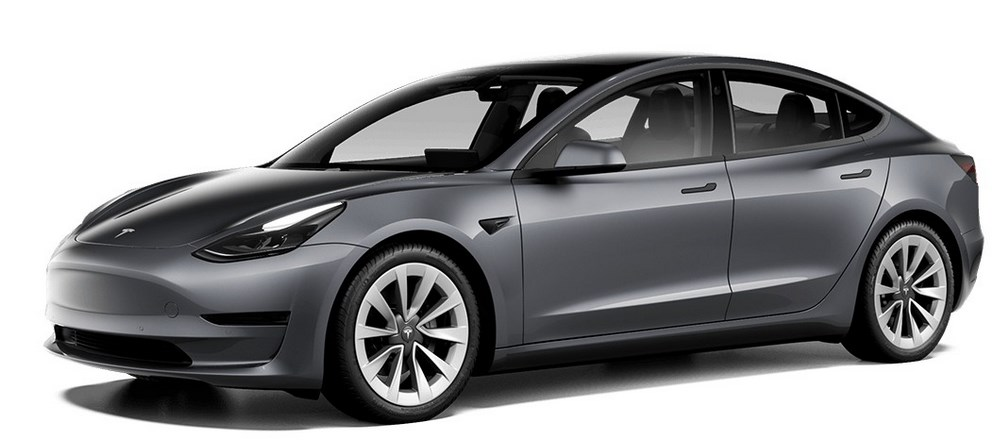
\includegraphics[width=0.9\columnwidth]{cars/tesla-model-3.jpg}

Tesla Model 3
\end{center}

\begin{itemize}
    \item LL/BJ: 0/2022, 5-Sitzer $\rightarrow$ Laufzeit: 7 Jahre
    \item \href{https://www.tesla.com/de_de/model3/design\#overview}{Weblink}
    \item \emph{Gesch\"atzter} Spritpreis \"uber Haltedauer: 0.31 \euro{}/kWh
    \item Antrieb: Strom, mit 325 PS
    \item Restwert nach Faustformel (Kaufpreis $\times$ 19.8\%): 8724.75 \euro{}
\end{itemize}

\begin{small}
\emph{Meinung Nataliya:} 0/10: 
        
\emph{Meinung Grzegorz:} 0/10: 
\end{small}

\pagebreak


\twocolumn

\section*{VW Touran Schw. Gd., neu, Benzin, Kredit}
\begin{center}
\includegraphics[width=0.5\textheight]{images1/vw-touran-schw-gd-n150kB7-boundaries_.png}
\null
\vspace{0.5cm}
\includegraphics[width=0.5\textheight]{images1/vw-touran-schw-gd-n150kB7-calc_df_.png}
\end{center}

\pagebreak
\begin{center}
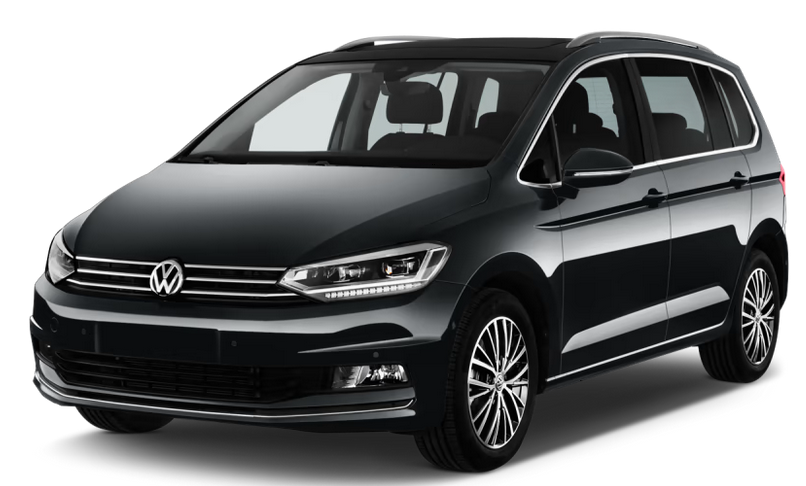
\includegraphics[width=0.9\columnwidth]{cars/vw-touran.png}

VW Touran Schw. Gd.
\end{center}

\begin{itemize}
    \item LL/BJ: 0/2022, 7-Sitzer $\rightarrow$ Laufzeit: 7 Jahre
    \item \href{https://www.volkswagen.de/de/konfigurator.html/__app/touran/touran/comfortline.app?buildabilityStatus-app=buildable&category-app=private&carlineId-app=31000&salesGroupId-app=32600&trimName-app=Comfortline&modelId-app=5T13PZ%24GYORYOR&modelVersion-app=3&modelYear-app=2022&exteriorId-app=F14+5K5K&interiorId-app=F56+++++VE&options-app=MSTD7B2-GPG4PG4-MESSU9C-GPJ9PJ9-GPF6PF6-GPKJPKJ-GPLLPLL-MHKAKH7-GWLLWLL-GWL2WL2-GPM3PM3-GRBDRBD-MTRW3CX-MKSUKA1-MSAB4X4-GP19P19-GWQ1WQ1-GWWCWWC}{Weblink}
    \item \emph{Gesch\"atzter} Spritpreis \"uber Haltedauer: 1.95 \euro{}/l
    \item Antrieb: Benzin, mit 150 PS
    \item Restwert nach Faustformel (Kaufpreis $\times$ 19.8\%): 7934.29 \euro{}
\end{itemize}

\begin{small}
\emph{Meinung Nataliya:} 9/10: Auto war ruhig. Hinten viel Platz, Auto ist nicht auf der Straße gehüpft,
                    gut gedämpft. Innen sehr hoch. Leicht zu bedienen, alles an seinem Platz. Rücksitz
                    war leichter zu erreichen als bei allen anderen. Sehr großer Kofferaum.
        
\emph{Meinung Grzegorz:} 9/10: War leider ein Handschalter, aber hat trotzdem spaß gemacht. 
                   Leises auto, bequeme Sitze, viel Platz. Hinten drei Sitze. Dritte Sitzreihe gut nutzbar.
                   Verbrauch auf Testfahrt annehmbar (8l/100km). Leichtgängige Lenkung, Fahrwerk hat Straße 
                   gut weggefedert.
\end{small}

\pagebreak



\pagebreak

\onecolumn
\begin{figure}
\centering
Vergleich der monatlichen Kosten bei \euro{} 10000.00 Anzahlung bei Kreditfinanzierung und \euro{} 3000.00 bei Leasing.

Gesch\"atzer Kraftstoffpreis: 1.95 \euro{}/l Benzin, 1.99 \euro{}/l Diesel bzw. 0.31 \euro{}/kWh


\vspace{1em}
\includegraphics[width=0.95\columnwidth]{images1/overview1.png}
\end{figure}
\vfill 



\end{document}
